% Author: Mathias Hablützel

\section{Erfassung Schiffsgeschwindigkeiten}

\subsection{Windangriffswinkel und Windgeschwindigkeit}

\begin{wrapfigure}{r}{6cm} 
\centering
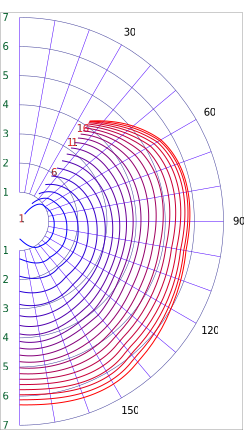
\includegraphics[width=6cm]{img/polardiagramm}
\caption{Polardiagramm eines Bootes, grün Windstärke in Knoten, rot
Geschwindigkeit in Knoten, schwarz Windangriffswinkel}
\label{polardiagram}
\end{wrapfigure}

Je nach Einfallswinkel des Windes variert die Schiffsgeschwindigkeit stark.
Bei frontal kommenden Wind\footnote{Im Segeljargon "im Wind" genannt, daher
der Wind fällt von Bug her ein.} fährt das Schiff gar nicht mehr vorwärts und
muss für diesen Umstand aufkreuzen, das heisst einen Zickzack-Kurs fahren.
Deshalb muss für jedes Schiff empirisch der minimale Einfallswinkels vom Bug
aus ermittelt werden, somit ist der steilste Winkel bekannt bevor die Segel
killen\footnote{Im Segeljargon bezeichnet "killen" das flattern der Segeln
ohne Vortrieb zu erzeugen.}.

Die Schiffsgeschwindigkeit variert aufgrund der physischen Eigenschaften von
Segel, Rumpf und Aerodynamik. Entgegen der Intuition ist ein Wind von
Achtern\footnote{Im Segeljargon bezeichnet "achtern" alles was ab Mittschiffs
hinten lieg.} nicht der schnellste, sondern bei sogenannt halben Wind (meist
zwischen 80\degree und 105\degree). Da sich diese Daten nicht nur bei
unterschiedlichen Einfallswinkel verändern, sondern auch bei unterschiedlichen
Windgeschwindigkeiten, empfiehlt es sich ein sogenanntes Polardiagramm zu
erstellen. So stell man die unterschiedlichen Fahrtgeschwindigkeiten in Bezug
zu Einfallswinkel und Windgeschwindigkeit dar.

Da aber der Datensatz nicht vollständig bekannt ist, muss zwischen den bekannten
und ermittelten Punkten interpoliert werden.

\subsection{Interpolationsverfahren}
Um diese Daten zu interpolieren eignet sich die bilineare Interpolation am
besten, da sie sehr einfach zu implementieren ist. Diese verfügt über eine für
unsere Zwecke genügend hohe Genauigkeit, rechnet in linearer Zeit und nur aus
Multiplikationen sowie Additionen besteht. Aufgrund von den heutigen
CPU-Befehlen nur noch wenigen Taktzyklen braucht und somit zu einer sehr hohen
Ausführgeschwindigkeit führt.

Andere Interpolationsmethoden wie kubische Interpolation, Spline-Interpolation
oder polynomielle Interpolation sind entweder zu aufwändig, langsam oder
instabil. Daher wurden diese Algorithmen nicht in Betracht gezogen. Ausserdem
verwendet die bilineare Interpolation nur die unmittelbaren Nachbarwerte und
kommt damit mit weniger Informationen zurecht.
